\documentclass[tikz]{standalone}
\usetikzlibrary{arrows, positioning}
\usetikzlibrary {arrows.meta}
\usepackage{xcolor}
\definecolor{allcolor}{RGB}{148,182,233}
\begin{document}
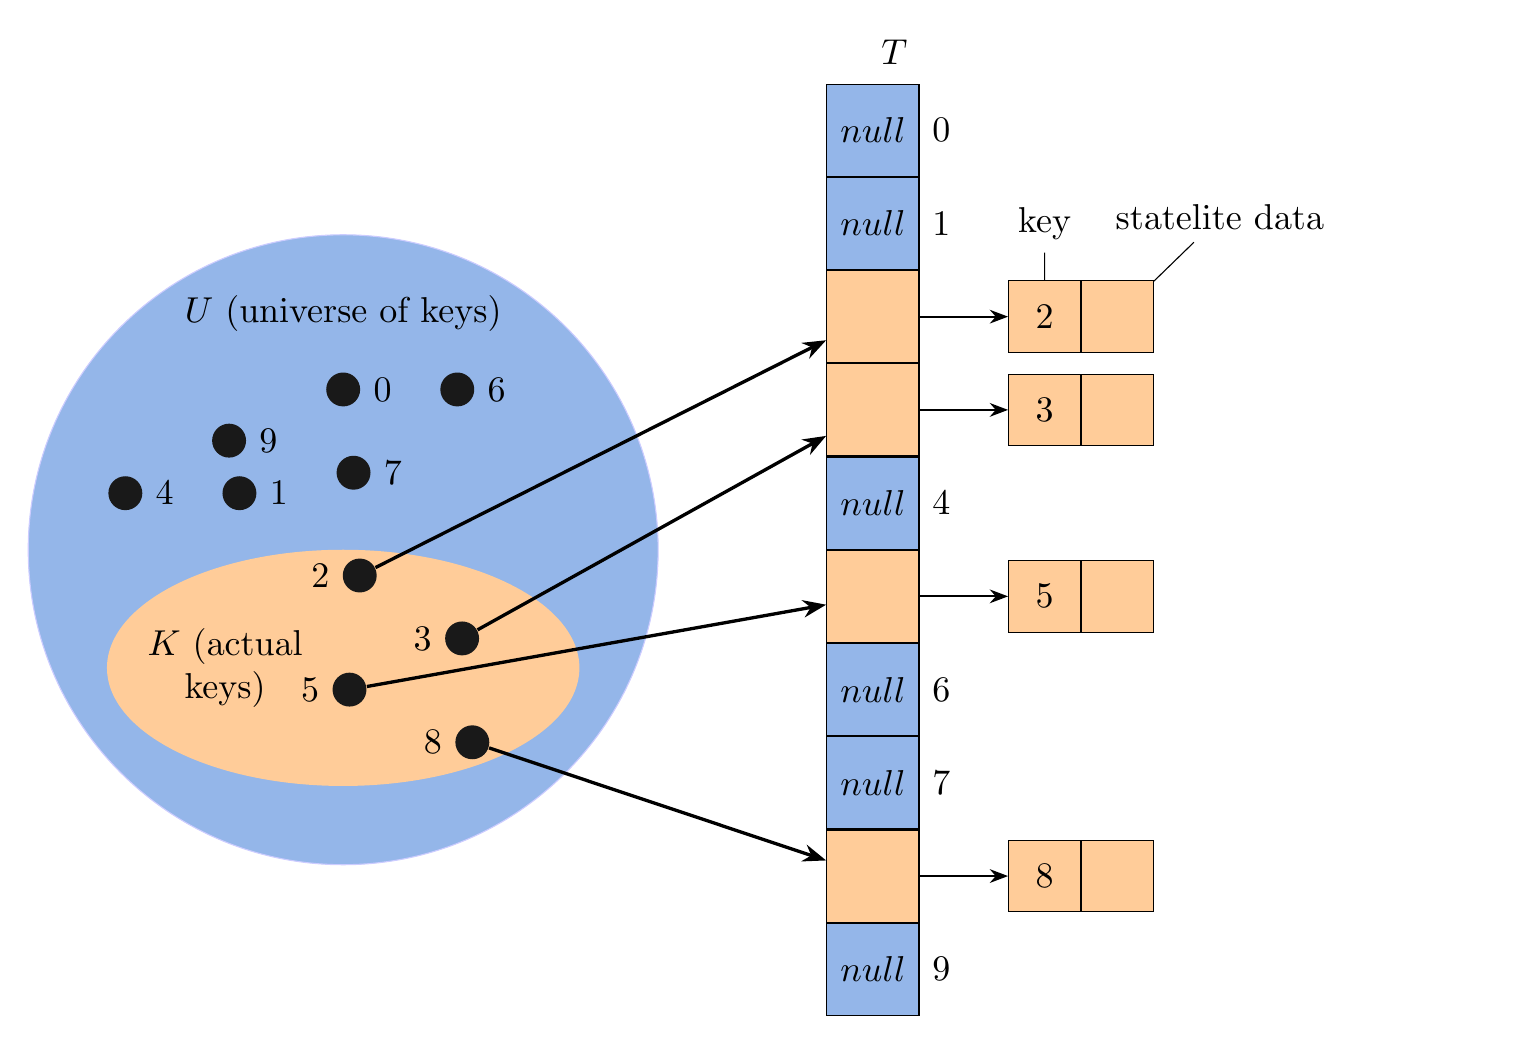
\begin{tikzpicture}[every node/.style={scale=1.3}, dot/.style={minimum size=0.1mm, circle, fill=black!90}, slot/.style={minimum size=0.9cm, rectangle}, noslot/.style={slot, fill=allcolor},
    yesslot/.style={slot, fill=orange!40}, data/.style={minimum size=0.7cm, fill=orange!40}, >=Stealth]
    \tikzstyle{textbf} = [text width=5cm,text centered]

    \filldraw[color=blue!20, fill=allcolor](0,0) circle (4);
    \node[textbf] (universe) at (0, 3) {$U$ (universe of keys)};
    
    \node[dot, label=right:$0$] [below=of universe, yshift=0.5cm] (i0) {};
    \node[dot, label=right:$6$] [right=of i0] {};
    \node[dot, label=right:$9$] [left=of i0, yshift=-0.5cm]{};
    \node[dot, label=right:$1$] [below left=of i0] (i1){};
    \node[dot, label=right:$4$] [left=of i1]{};
    \node[dot, label=right:$7$] [right=of i1,yshift=0.2cm]{}; 

    \fill[orange!40] (0, -1.5) ellipse (3 and 1.5);
    \node[textbf, text width=2cm] (keys) at (-1.5, -1.5) {$K$ (actual keys)};

    \node[dot, label=left:$2$] [above right=of keys, xshift=-0.7cm, yshift=-0.5cm] (i2){};
    \node[dot, label=left:$3$, xshift=1cm, yshift=0.5cm] [below=of i2] (i3){};
    \node[dot, label=left:$5$] [below=of i2, xshift=-0.1cm] (i5){};
    \node[dot, label=left:$8$] [below=of i3, yshift=0.1cm, xshift=0.1cm] (i8){};

    \matrix [column sep=1cm,nodes=draw] (table) at (7, 0)
    {
      \node[noslot, label=right:$0$] {$null$}; \\
      \node[noslot, label=right:$1$] {$null$}; \\
      \node[yesslot] (s2) {}; \\
      \node[yesslot] (s3) {}; \\
      \node[noslot, label=right:$4$] {$null$}; \\
      \node[yesslot] (s5) {}; \\
      \node[noslot, label=right:$6$] {$null$}; \\
      \node[noslot, label=right:$7$] {$null$}; \\
      \node[yesslot] (s8) {}; \\
      \node[noslot, label=right:$9$] {$null$}; \\
    };

    \node[textbf, above=of table,yshift=-0.8cm]{$T$};
    \draw[->, very thick]  (i2) to (s2);
    \draw[->, very thick]  (i3) to (s3); 
    \draw[->, very thick]  (i5) to (s5);
    \draw[->, very thick] (i8) to (s8);


    \matrix [nodes=draw, right=of s2] (data2)
    {
      \node[data] (k2) {2}; & \node[data] (v2) {}; \\
    };

    \node[textbf][above=of k2, yshift=-0.5cm] (keyinfo) {key};
    \node[textbf][above=of v2, xshift=1cm,yshift=-0.4cm] (valueinfo) {statelite data};
    \draw (keyinfo) to (k2);
    \draw (valueinfo) to (v2);

    \draw[->, thick] (s2) to (k2);

    \matrix [nodes=draw, right=of s3]
    {
      \node[data] (k3) {3}; & \node[data]  {}; \\
    };

    \draw[->, thick] (s3) to (k3);

    \matrix [nodes=draw, right=of s5]
    {
      \node[data] (k5) {5}; & \node[data]  {}; \\
    };

    \draw[->, thick] (s5) to (k5);

    \matrix [nodes=draw, right=of s8]
    {
      \node[data] (k8) {8}; & \node[data]  {}; \\
    };

    \draw[->, thick] (s8) to (k8);
    
\end{tikzpicture}
\end{document}